\chapter{Neutrino detection\label{chap:nu-detection}}
In order to be able to detect particles, they need to interact with a detection medium.
This chapter will describe the most important interaction of charged particles as well as neutral particles with matter.
A special focus is laid on charged interactions as these are the most important ones for \lartpc s.
As a measure of the interaction strength, the energy loss per distance or stopping power $\frac{\m{d}E}{\m{d}x}$ is used.
Where not otherwise mentioned, this chapter is based on~\cite{grupen}.


\section{Charged particles\label{sec:interaction_charged_particles}}
The main interaction of charged particles with matter happens on atomic electrons.
That is why for most of these interactions, one needs to treat the interaction of electrons separately.
For all other charged particles, the stopping power is described by the Bethe-Bloch formula
\begin{IEEEeqnarray}{rCl}
	- \frac{1}{\rho} \dv{E}{x} & = &
	4 \pi N_{\m{A}} r_{\m{e}} ^ 2 m_{\m{e}} c ^ 2 z ^ 2 \frac{Z}{A} \frac{1}{\beta ^ 2}
	\qty[\ln(\frac{2 m_{\m{e}} c ^ 2 \gamma ^ 2 \beta ^ 2}{I}) - \beta ^ 2 - \frac{\delta}{2}] \m{,}
	\label{eq:bethe-bloch}
\end{IEEEeqnarray}
where
\begin{itemize}
	\item[$\rho$] is the density of the absorber material,
	\item[$N_{\m{A}}$] is Avogadro's number,
	\item[$r_{\m{e}}$] $= \frac{1}{4 \pi \varepsilon_{\m{0}}} \frac{\si{\elementarycharge} ^ 2}{m_{\m{e}} c ^ 2}$ is the classical electron radius using the permittivity of free space $\varepsilon_{\m{0}}$,
	\item[$m_{\m{e}}$] is the electron mass,
	\item[$z$] is the charge of the incident particle,
	\item[$Z$] is the atomic number of the absorber,
	\item[$A$] is the atomic weight of the absorber,
	\item[$\beta$] $= \frac{v}{c}$ with $v$ the velocity of the incident particle,
	\item[$\gamma$] $= \frac{E}{m_0 c ^ 2}$ with $E$ the energy and $m_0$ the rest mass of the incident particle,
	\item[$I$] is the mean excitation energy of the absorber material which can be approximated by
		\begin{IEEEeqnarray}{rCl}
			I = 16 Z ^ {0.9} \si{\electronvolt} \quad \m{for} \quad Z > 1 \m{,}
		\end{IEEEeqnarray}
	\item[$\delta$] is a parameter describing the screening of the extended transverse electric field of relativistic incident particles by the charge density of the atomic electrons of the absorber.
\end{itemize}
Equation~\eqref{eq:bethe-bloch} describes the stopping power of particles with $m_0 \gg m_{\m{e}}$ by ionisation and excitation of the atoms in the absorber material.
As the stopping power is proportional to the electron density and thus to the mass density of the absorber material, it is often divided by the latter.
Thus, Equation~\eqref{eq:bethe-bloch} actually gives the so called mass stopping power.
The only remaining dependence on the absorber material is $\frac{Z}{A}$ which is $\approx 0.5$ for most light materials, and the mean excitation energy which only contributes logarithmically.
\begin{figure}[htbp]
	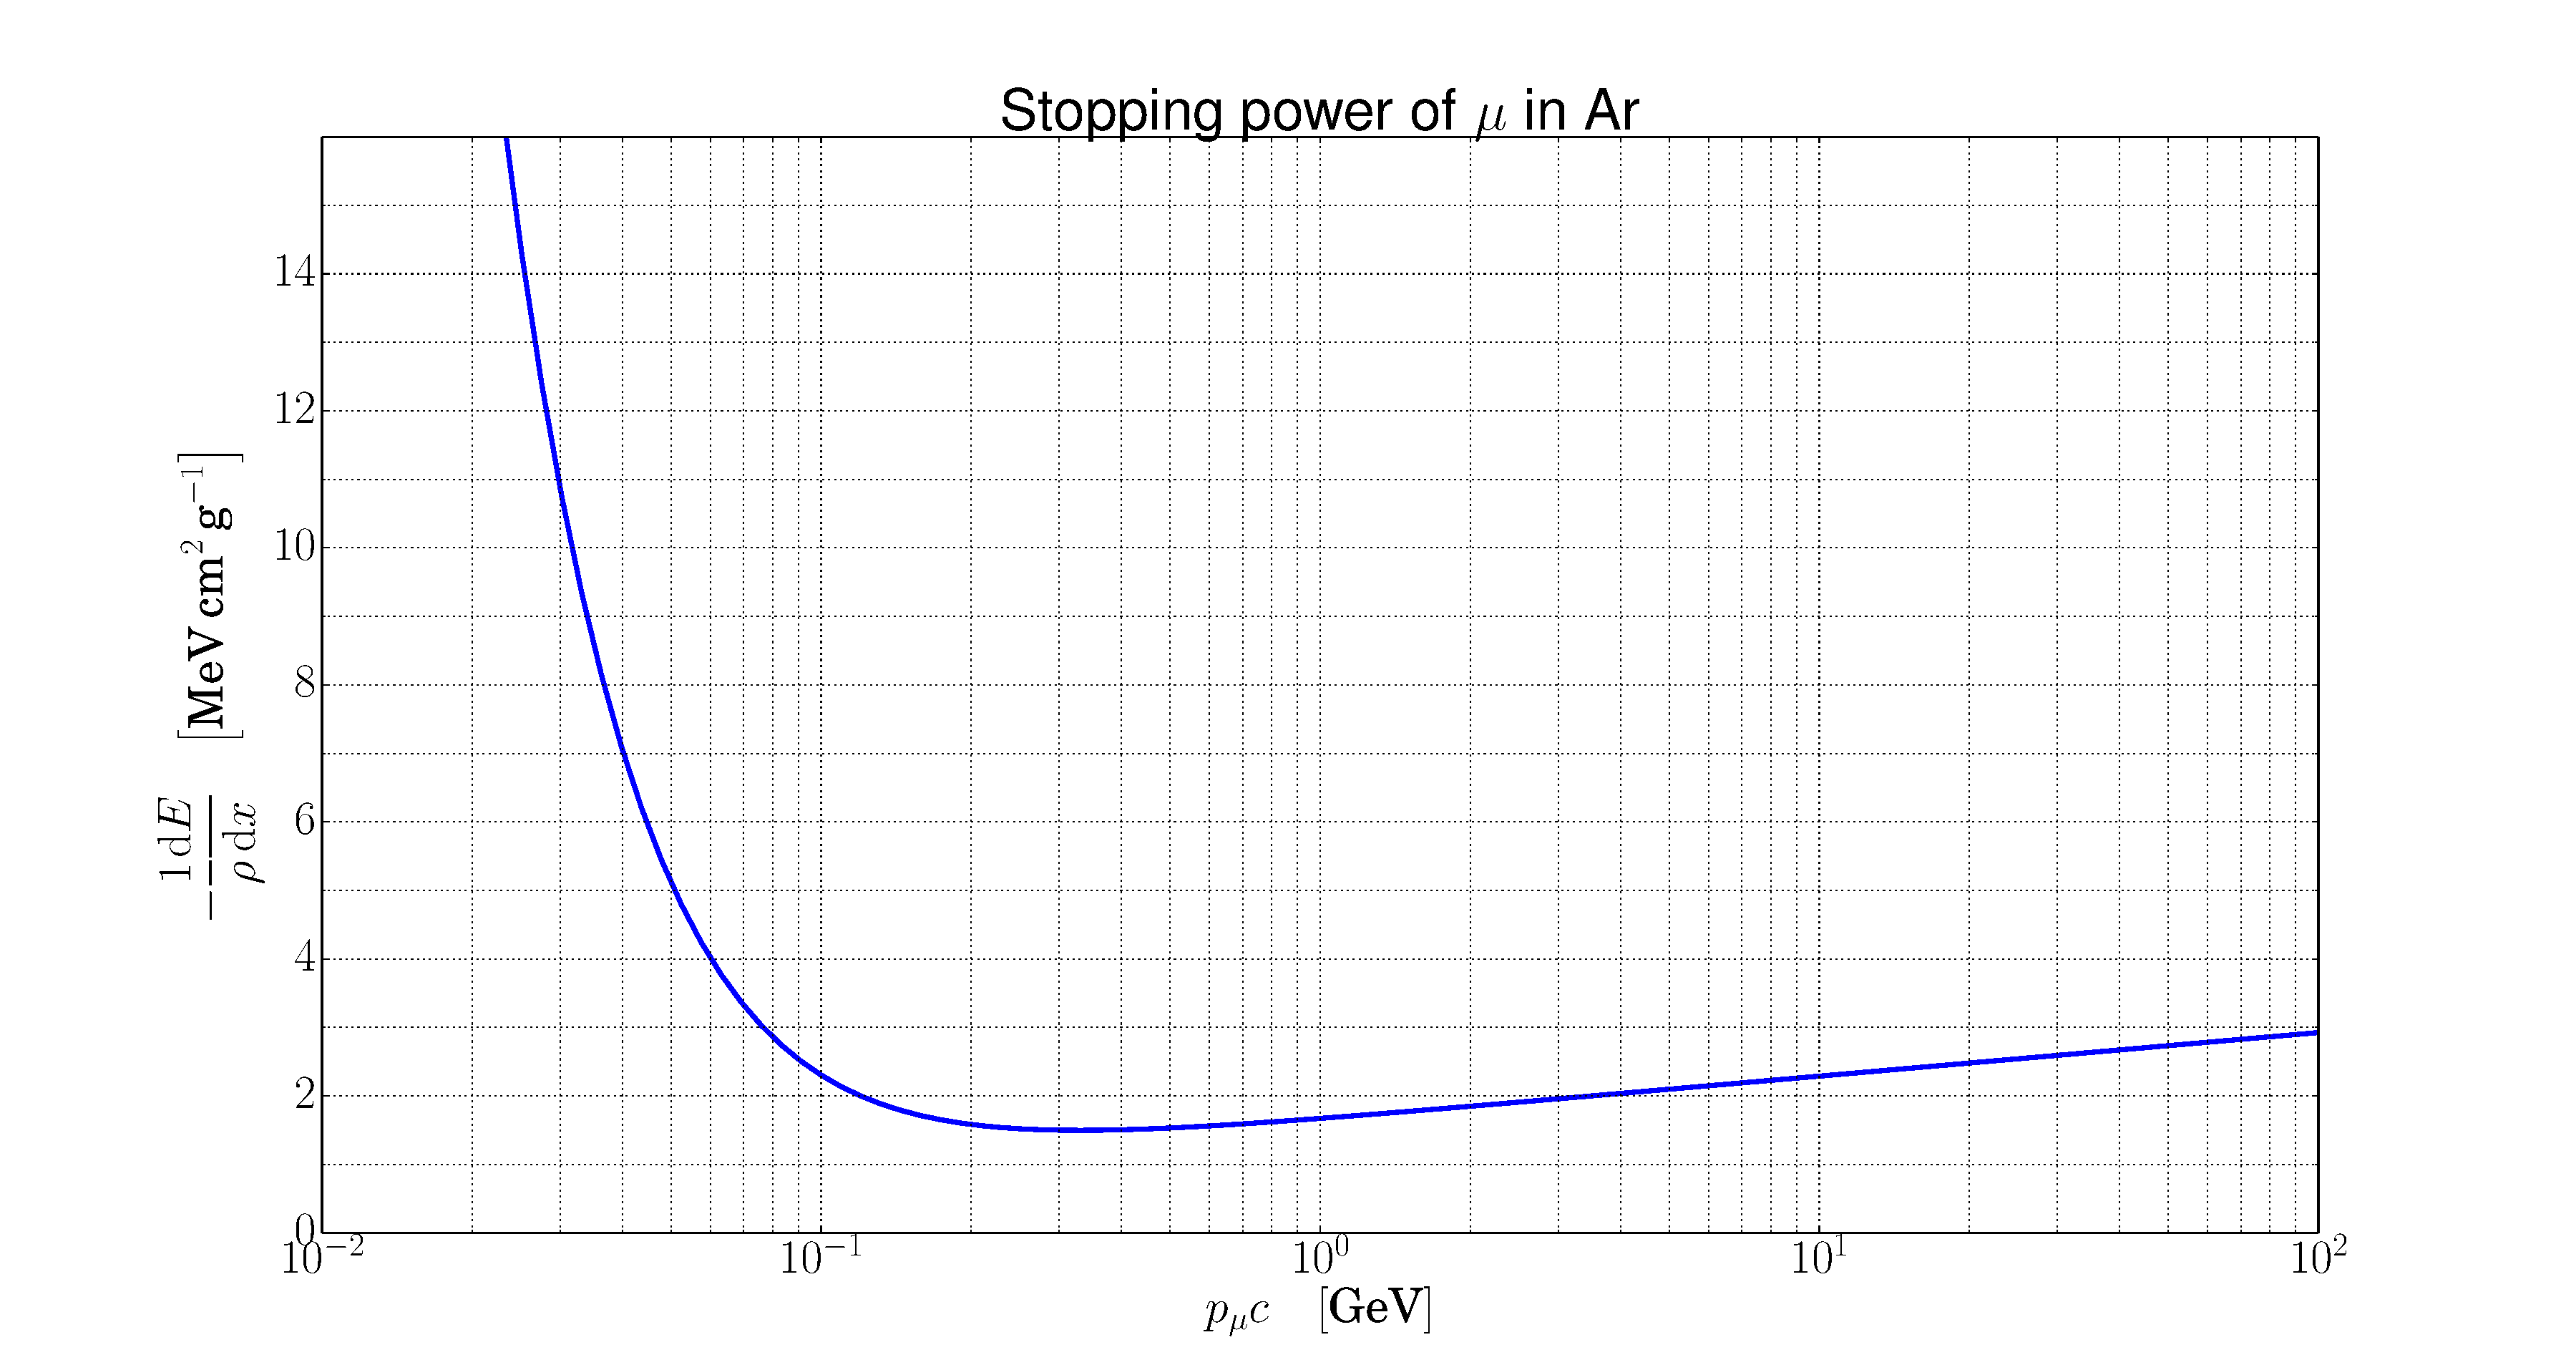
\includegraphics[width=\textwidth]{bethe-bloch}
	\caption{Bethe-Bloch stopping power of $\mu$ in \si{Fe}\label{fig:bethe-bloch}}
\end{figure}
Figure~\ref{fig:bethe-bloch} shows the mass stopping power of $\mu$ in \si{Fe} neglecting the $\frac{\delta}{2}$ term.
As can be seen, there is a broad minimum which is characteristic of the Bethe-Bloch formula.
Particles in this momentum range are called minimum ionising particles (MIPs).
They are important for detectors because this energy loss is a measure for the required energy resolution of a detector.
As mentioned above, the mass stopping power only loosely depends on the absorber material and therefore, its minimum is
\begin{IEEEeqnarray}{rCl}
	\eval{- \frac{1}{\rho} \dv{E}{x}}_{\m{min}} & \approx & \SI{2}{\mega\electronvolt\centi\meter\squared\per\gram}
\end{IEEEeqnarray}
for singly charged incident particles on most (light) absorbers.
To the left of the minimum is the \emph{Bragg peak} which is especially important for radiation therapy with heavy charged particles (e.g.\ protons).
The Bragg peak falls off with a strong $\frac{1}{\beta ^ 2}$ dependence.
After the minimum, the stopping power rises again with a logarithmic dependence on $\beta$ and the mean excitation energy of the absorber $I$.
The reason for this so called \emph{logarithmic rise} is the extension of the transverse electric field of the incident particle in the relativistic regime.
Due to increasing shielding of the transverse electric field by the shell electrons of the absorber materials, taken into account by the $\frac{\delta}{2}$ term, the rise is only asymptotic.
For electrons and positrons, Equation~\eqref{eq:bethe-bloch} does not hold because their mass is equal to the mass of the atomic electrons of the absorber.
The stopping power changes further for electrons because the incident particle cannot be distinguished form its collision partner in that case.
On the other hand, a positron will be annihilated upon stop by an electron which needs to be taken into account as well.
The equivalent of Equation~\eqref{eq:bethe-bloch} for $e^{\pm}$ can be found in~\cite{grupen}.

At high velocities, further effects come into play.
\emph{Bremsstrahlung} describes the radiation energy loss of a fast charged particle in the Coulomb field of the absorber nuclei.
It can be described by
\begin{IEEEeqnarray}{rCl}
	- \frac{1}{\rho}\dv{E}{x} & = & \frac{E}{X_{\m{0}}}
	\label{eq:bremsstrahlung}
\end{IEEEeqnarray}
where
\begin{IEEEeqnarray}{rCl}
	X_{\m{0}} & = & \frac{A}{4 \alpha N_A Z \qty(Z + 1) \qty(\frac{1}{4 \pi \varepsilon_{\m{0}}} \frac{\si{\elementarycharge} ^ 2}{m c ^ 2}) ^ 2 \ln(183 Z ^ {- \frac{1}{3}})}
	\label{eq:radiationlength}
\end{IEEEeqnarray}
is the \emph{radiation length} of the absorber material using
\begin{itemize}
	\item[$\alpha$] $\approx \frac{1}{137}$ the fine-structure constant and
	\item[$m$] the mass of the incident particle.
\end{itemize}
Again, the energy loss is proportional to the density of the absorber and for convenience, divided by the latter.
Bremsstrahlung is emitted in interactions of the incident particle with the absorber nuclei ($\propto Z ^ 2$) as well as with the atomic electrons of the absorber ($\propto Z$).
By neglecting the latter, one obtains the important relation
\begin{IEEEeqnarray}{rCl}
	X_0 ^ {- 1} & \propto & Z ^ 2
\end{IEEEeqnarray}
as opposed to the $\propto Z$ dependence of the Bethe-Bloch formula.
Equation~\eqref{eq:bremsstrahlung} also holds for electrons as long as $E \gg \frac{m_{\m{e}} c ^ 2}{\alpha Z ^ {\frac{1}{3}}}$.
Furthermore, looking at the dependence on the mass of the incident particle, one finds
\begin{IEEEeqnarray}{rCl}
	X_0 & \propto & m ^ 2
\end{IEEEeqnarray}
using Equation~\eqref{eq:radiationlength}.
Therefore, the radiation length of an absorber material is usually given for electrons and the relation
\begin{IEEEeqnarray}{rCl}
	X_0 & = & X_0^{\m{e}} \frac{m ^ 2}{m_{\m{e}} ^ 2}
\end{IEEEeqnarray}
can be used to get the radiation length for any charged particle of mass $m$.
Radiation losses play a significant role only at energies much higher than the energy of MIPs.
Using Equations~\eqref{eq:bethe-bloch} and~\eqref{eq:bremsstrahlung}, one can define a \emph{critical energy} $E_{\m{c}}$ by
\begin{IEEEeqnarray}{rCl}
	\eval{\dv{E}{x}_{\m{ion}}}_{E_{\m{c}}} & = & \eval{\dv{E}{x}_{\m{brems}}}_{E_{\m{c}}}
\end{IEEEeqnarray}
at which radiation losses take over from ionisation losses.
Similar to the radiation length, the critical energy is proportional to $m ^ 2$.
Thus, it is most important for electrons while for other particles it becomes significant only at very high energies.
If we take the example of an iron absorber again for instance, we get $E_c^{\m{e}} = \SI{20.7}{\mega\electronvolt}$ and $E_c^{\mu} = \SI{890}{\giga\electronvolt}$.

At high energies, there are additional types of radiation loss taking place, for instance direct electron-pair production and photonuclear interactions.
They shall not be described here.
Instead, only their $\propto E$ relation similar to bremsstrahlung losses shall be mentioned.
A description of those effects can be found in~\cite{grupen}.

Concerning the interactions of charged particles with matter, there is one important note regarding detectors.
While charge produced in interactions (i.e.\ ionisation) can be detected directly, light (i.e.\ excitation photons and photon radiation) first needs to be converted to charge to be detected.
This conversion from light to electric charge is the topic of the next section.


\section{Photons\label{sec:interaction_photons}}
Photons can interact with matter in different ways.
In particular, they can be converted to charge which can be detected.
The three most important interactions converting photons to charge shall be outlined in this section.
All of them have in common that they attenuate photon beams exponentially according to
\begin{IEEEeqnarray}{rCl}
	I & = & I_0 \m{e} ^ {- \mu x}
\end{IEEEeqnarray}
where $I_0$ and $I$ is the intensity before and after passing the absorber, respectively.
The thickness of the absorber is given by $x$ and
\begin{IEEEeqnarray}{rCl}
	\mu & = & \frac{N_A}{A} \sum_i \sigma_i
	\label{eq:mass_att_coeff}
\end{IEEEeqnarray}
is the \emph{mass attenuation coefficient} defined by the sum of the cross sections $\sigma_i$ of the different interaction processes.

At low energies (ionisation energy $\le E_{\gamma} \le \SI{100}{\kilo\electronvolt}$), photons primarily undergo conversion to charge by the \emph{photoelectric effect}.
The photon is absorbed by an atom of the absorber which in turn is ionised and thus ejects one of its shell electrons.
The cross section is given by
\begin{IEEEeqnarray}{rCl}
	\sigma_{\m{photo}} = \qty(\frac{32}{\epsilon ^ 7}) ^ \frac{1}{2} \alpha ^ 4 Z ^ 5 \sigma_{\m{Th}}^{\m{e}}
\end{IEEEeqnarray}
where
\begin{itemize}
	\item[$\epsilon$] $= \frac{E_{\m{\gamma}}}{m_{\m{e}} c ^ 2}$ is the reduced photon energy and
	\item[$\sigma_{\m{Th}}^{\m{e}}$] $= \frac{8}{3} \pi r_{\m{e}} ^ 2 = \SI{6.65e-25}{\centi\meter\squared}$ is the \emph{Thomson cross section} for elastic scattering of photons on electrons.
\end{itemize}

For energies $\approx \SI{1}{\mega\electronvolt}$, \emph{Compton scattering} dominates the interaction of photons with matter.
Thereby, the photon is not absorbed by the atom but just scatters off one of its shell electrons with the cross section
\begin{IEEEeqnarray}{rCl}
	\sigma_{\m{c}} & = & 2 \pi r_{\m{e}} ^ 2 Z \left\{\qty[\frac{1 + \epsilon}{\epsilon ^ 2}] \qty[\frac{2 \qty(1 + \epsilon)}{1 + 2 \epsilon} - \frac{1}{\epsilon} \ln(1 + 2 \epsilon)]\right.\\
	& & \left. + \frac{1}{2 \epsilon} \ln(1 + 2 \epsilon) - \frac{1 + 3 \epsilon}{\qty(1 + 2 \epsilon) ^ 2}\right\}
\end{IEEEeqnarray}
obtained from the Klein-Nishina formula.
As only part of the photon's energy is absorbed while the rest is scattered, it makes sense to divide this cross section into a scattering cross section
\begin{IEEEeqnarray}{rCl}
	\sigma_{\m{cs}} & = & \frac{E_{\gamma}'}{E_{\gamma}}
\end{IEEEeqnarray}
and an absorption cross section
\begin{IEEEeqnarray}{rCl}
	\sigma_{\m{ca}} & = & \sigma_{\m{c}} - \sigma_{\m{cs}}
\end{IEEEeqnarray}
where $E_{\gamma}$ and $E_{\gamma}'$ is the energy of the photon before and after scattering, respectively.

At $E_{\gamma} \ge 2 m_{\m{e}} c ^ 2$, photons are capable of producing pairs of $e^+ e^-$.
Because of momentum conservation, this process can only happen in the coulomb field of a so called spectator particle.
As pair-production in the field of an electron is strongly suppressed, the spectator is usually a nucleus of the absorber material.
Therefore, the cross section of pair-production depends on the shielding of the coulomb field by the shell electrons and thus on the proximity to the nucleus.
Eventually, this results in an energy dependence.
For $1 \ll \epsilon < \frac{1}{\alpha Z ^ {\frac{1}{3}}}$, the cross section is given by
\begin{IEEEeqnarray}{rCl}
	\sigma_{\m{pair}} & = & 4 \alpha r_{\m{e}} ^ 2 Z ^ 2 \qty(\frac{7}{9} \ln 2 \epsilon - \frac{109}{54})
\end{IEEEeqnarray}
and for $\epsilon \gg \frac{1}{\alpha Z ^ {\frac{1}{3}}}$, the cross section is
\begin{IEEEeqnarray}{rCl}
	\sigma_{\m{pair}} & = & 4 \alpha r_{\m{e}} ^ 2 Z ^ 2 \qty[\frac{7}{9} \ln(\frac{183}{Z ^ {\frac{1}{3}}}) - \frac{1}{54}] \m{.}
\end{IEEEeqnarray}

As mentioned above, for Compton scattering, two different cross sections are defined, one for the scattered energy ($\sigma_{\m{cs}}$) and one for the absorbed one ($\sigma_{\m{ca}}$).
Consequentially, there are also different definitions of the coefficient $\mu$ in Equation~\eqref{eq:mass_att_coeff}.
Replacing $\sigma_{\m{c}}$ by $\sigma_{\m{cs}}$, $\mu_{\m{s}}$ is the \emph{mass attenuation coefficient} and similarly, using $\sigma_{\m{ca}}$, $\mu_{\m{s}}$ is the \emph{mass absorption coefficient}.
While $\mu$ is more precisely called the \emph{total mass attenuation coefficient}.


\section{Hadrons\label{sec:interactions_hadrons}}